\documentclass{standalone}
\usepackage{tikz}
\usetikzlibrary{patterns, positioning}


\begin{document}
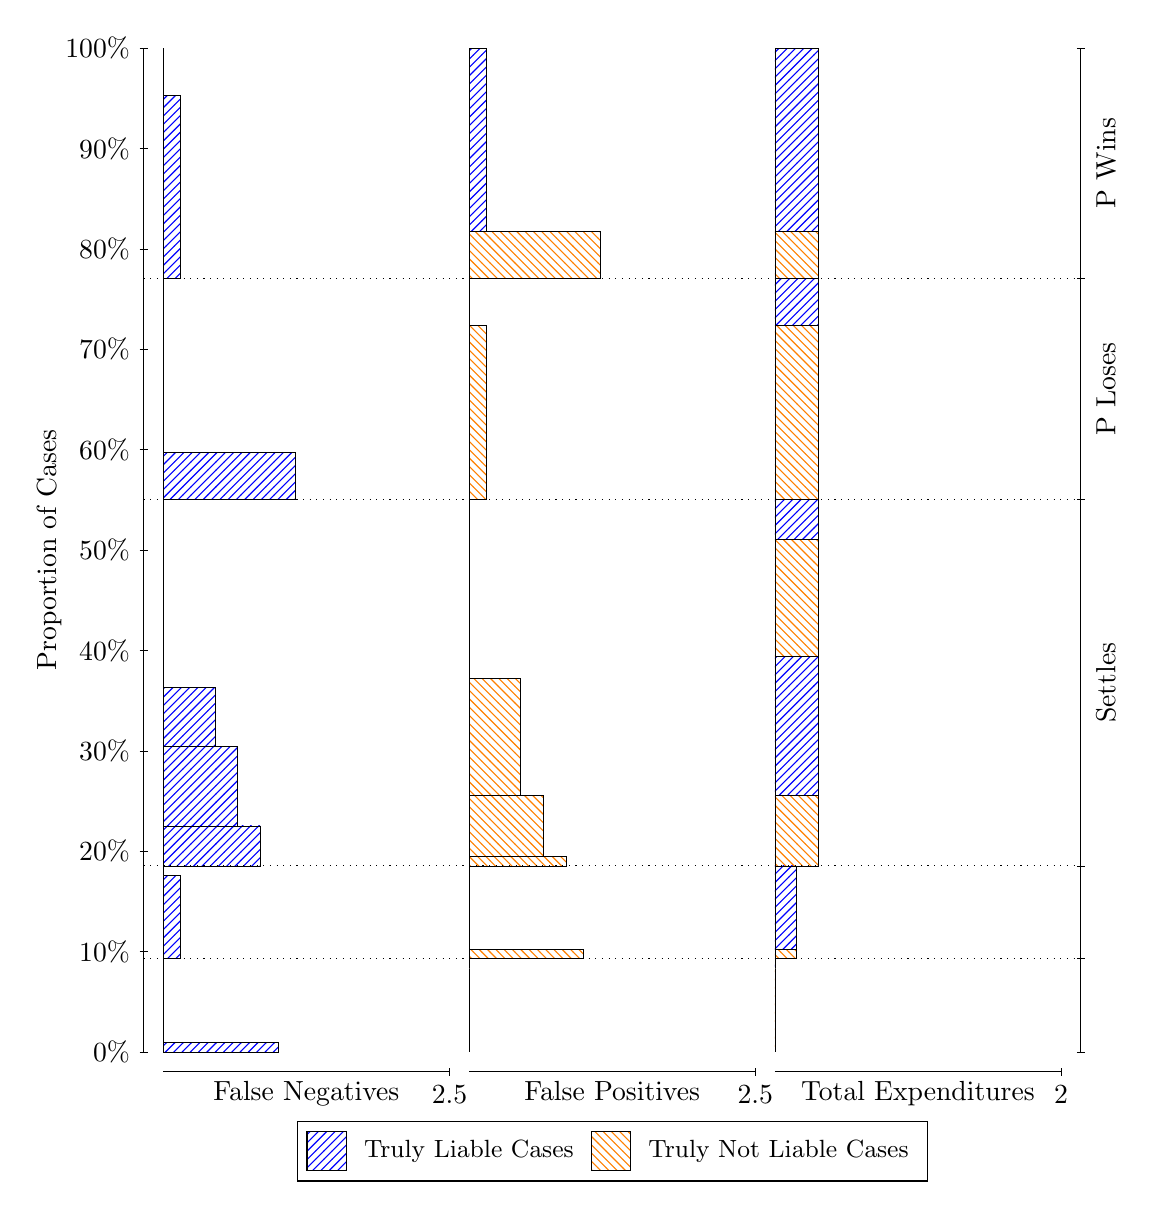
\begin{tikzpicture}
\draw[black, very thin] (1.5,1.75) -- (1.5,14.5);
\node[rotate=90, text=black, anchor=center] at (0.3, 8.125) {Proportion of Cases};
\draw[black, very thin] (1.45,1.75) -- (1.55,1.75);
\node[text=black, anchor=east] at (1.45, 1.75) {0\%};
\draw[black, very thin] (1.45,3.025) -- (1.55,3.025);
\node[text=black, anchor=east] at (1.45, 3.025) {10\%};
\draw[black, very thin] (1.45,4.3) -- (1.55,4.3);
\node[text=black, anchor=east] at (1.45, 4.3) {20\%};
\draw[black, very thin] (1.45,5.575) -- (1.55,5.575);
\node[text=black, anchor=east] at (1.45, 5.575) {30\%};
\draw[black, very thin] (1.45,6.85) -- (1.55,6.85);
\node[text=black, anchor=east] at (1.45, 6.85) {40\%};
\draw[black, very thin] (1.45,8.125) -- (1.55,8.125);
\node[text=black, anchor=east] at (1.45, 8.125) {50\%};
\draw[black, very thin] (1.45,9.4) -- (1.55,9.4);
\node[text=black, anchor=east] at (1.45, 9.4) {60\%};
\draw[black, very thin] (1.45,10.675) -- (1.55,10.675);
\node[text=black, anchor=east] at (1.45, 10.675) {70\%};
\draw[black, very thin] (1.45,11.95) -- (1.55,11.95);
\node[text=black, anchor=east] at (1.45, 11.95) {80\%};
\draw[black, very thin] (1.45,13.225) -- (1.55,13.225);
\node[text=black, anchor=east] at (1.45, 13.225) {90\%};
\draw[black, very thin] (1.45,14.5) -- (1.55,14.5);
\node[text=black, anchor=east] at (1.45, 14.5) {100\%};

\draw[black, very thin] (13.4,1.75) -- (13.4,14.5);
\draw[black, very thin] (13.35,1.75) -- (13.45,1.75);
\node[anchor=west] at (13.35, 1.75) {};
\draw[black, very thin] (13.35,2.9362) -- (13.45,2.9362);
\node[anchor=west] at (13.35, 2.9362) {};
\draw[black, very thin] (13.35,4.1137) -- (13.45,4.1137);
\node[anchor=west] at (13.35, 4.1137) {};
\draw[black, very thin] (13.35,8.7662) -- (13.45,8.7662);
\node[anchor=west] at (13.35, 8.7662) {};
\draw[black, very thin] (13.35,11.577) -- (13.45,11.577);
\node[anchor=west] at (13.35, 11.577) {};
\draw[black, very thin] (13.35,14.5) -- (13.45,14.5);
\node[anchor=west] at (13.35, 14.5) {};

\draw[black, very thin, pattern color=blue, pattern=north east lines] (1.75,1.75) rectangle (3.2033,1.8748);
\draw[black, very thin, pattern color=orange, pattern=north west lines] (1.75,1.8748) rectangle (1.75,2.9362);
\draw[black, very thin, pattern color=blue, pattern=north east lines] (1.75,2.9362) rectangle (1.968,3.9932);
\draw[black, very thin, pattern color=orange, pattern=north west lines] (1.75,3.9932) rectangle (1.75,4.1137);
\draw[black, very thin, pattern color=blue, pattern=north east lines] (1.75,4.1137) rectangle (2.9853,4.6213);
\draw[black, very thin, pattern color=blue, pattern=north east lines] (1.75,4.6213) rectangle (2.6947,5.6295);
\draw[black, very thin, pattern color=blue, pattern=north east lines] (1.75,5.6295) rectangle (2.404,6.3843);
\draw[black, very thin, pattern color=orange, pattern=north west lines] (1.75,6.3843) rectangle (1.75,8.7662);
\draw[black, very thin, pattern color=blue, pattern=north east lines] (1.75,8.7662) rectangle (3.4213,9.3639);
\draw[black, very thin, pattern color=orange, pattern=north west lines] (1.75,9.3639) rectangle (1.75,11.577);
\draw[black, very thin, pattern color=blue, pattern=north east lines] (1.75,11.577) rectangle (1.968,13.902);
\draw[black, very thin, pattern color=orange, pattern=north west lines] (1.75,13.902) rectangle (1.75,14.5);
\draw[black, very thin, pattern color=orange, pattern=north west lines] (5.6333,1.75) rectangle (5.6333,2.8114);
\draw[black, very thin, pattern color=blue, pattern=north east lines] (5.6333,2.8114) rectangle (5.6333,2.9362);
\draw[black, very thin, pattern color=orange, pattern=north west lines] (5.6333,2.9362) rectangle (7.0867,3.0567);
\draw[black, very thin, pattern color=blue, pattern=north east lines] (5.6333,3.0567) rectangle (5.6333,4.1137);
\draw[black, very thin, pattern color=orange, pattern=north west lines] (5.6333,4.1137) rectangle (6.8687,4.2332);
\draw[black, very thin, pattern color=orange, pattern=north west lines] (5.6333,4.2332) rectangle (6.578,5.0132);
\draw[black, very thin, pattern color=orange, pattern=north west lines] (5.6333,5.0132) rectangle (6.2873,6.4957);
\draw[black, very thin, pattern color=blue, pattern=north east lines] (5.6333,6.4957) rectangle (5.6333,8.7662);
\draw[black, very thin, pattern color=orange, pattern=north west lines] (5.6333,8.7662) rectangle (5.8513,10.979);
\draw[black, very thin, pattern color=blue, pattern=north east lines] (5.6333,10.979) rectangle (5.6333,11.577);
\draw[black, very thin, pattern color=orange, pattern=north west lines] (5.6333,11.577) rectangle (7.3047,12.175);
\draw[black, very thin, pattern color=blue, pattern=north east lines] (5.6333,12.175) rectangle (5.8513,14.5);
\draw[black, very thin, pattern color=orange, pattern=north west lines] (9.5167,1.75) rectangle (9.5167,2.8114);
\draw[black, very thin, pattern color=blue, pattern=north east lines] (9.5167,2.8114) rectangle (9.5167,2.9362);
\draw[black, very thin, pattern color=orange, pattern=north west lines] (9.5167,2.9362) rectangle (9.7892,3.0567);
\draw[black, very thin, pattern color=blue, pattern=north east lines] (9.5167,3.0567) rectangle (9.7892,4.1137);
\draw[black, very thin, pattern color=orange, pattern=north west lines] (9.5167,4.1137) rectangle (10.062,5.0132);
\draw[black, very thin, pattern color=blue, pattern=north east lines] (9.5167,5.0132) rectangle (10.062,6.7762);
\draw[black, very thin, pattern color=orange, pattern=north west lines] (9.5167,6.7762) rectangle (10.062,8.2586);
\draw[black, very thin, pattern color=blue, pattern=north east lines] (9.5167,8.2586) rectangle (10.062,8.7662);
\draw[black, very thin, pattern color=orange, pattern=north west lines] (9.5167,8.7662) rectangle (10.062,10.979);
\draw[black, very thin, pattern color=blue, pattern=north east lines] (9.5167,10.979) rectangle (10.062,11.577);
\draw[black, very thin, pattern color=orange, pattern=north west lines] (9.5167,11.577) rectangle (10.062,12.175);
\draw[black, very thin, pattern color=blue, pattern=north east lines] (9.5167,12.175) rectangle (10.062,14.5);
\draw[black, dotted] (1.5,2.9362) -- (13.4,2.9362);
\draw[black, dotted] (1.5,4.1137) -- (13.4,4.1137);
\draw[black, dotted] (1.5,8.7662) -- (13.4,8.7662);
\draw[black, dotted] (1.5,11.577) -- (13.4,11.577);
\draw[black, very thin] (1.75,1.5) -- (5.3833,1.5);
\node[text=black, anchor=north] at (3.5667, 1.5) {False Negatives};
\draw[black, very thin] (5.3833,1.45) -- (5.3833,1.55);
\node[text=black, anchor=north] at (5.3833, 1.45) {2.5};

\draw[black, very thin] (5.6333,1.5) -- (9.2667,1.5);
\node[text=black, anchor=north] at (7.45, 1.5) {False Positives};
\draw[black, very thin] (9.2667,1.45) -- (9.2667,1.55);
\node[text=black, anchor=north] at (9.2667, 1.45) {2.5};

\draw[black, very thin] (9.5167,1.5) -- (13.15,1.5);
\node[text=black, anchor=north] at (11.333, 1.5) {Total Expenditures};
\draw[black, very thin] (13.15,1.45) -- (13.15,1.55);
\node[text=black, anchor=north] at (13.15, 1.45) {2};



\node[text=black, centered, rotate=90] at (13.72, 6.44) {Settles};
\node[text=black, centered, rotate=90] at (13.72, 10.172) {P Loses};
\node[text=black, centered, rotate=90] at (13.72, 13.039) {P Wins};

\draw (7.449999999999999,1.5) node[draw=none] (baseCoordinate) {};
\begin{scope}[align=center]
        \matrix[scale=0.5, draw=black, below=0.5cm of baseCoordinate, nodes={draw}, column sep=0.1cm]{
            \node[rectangle, draw, minimum width=0.5cm, minimum height=0.5cm, pattern color=blue, pattern=north east lines] {}; &
            \node[draw=none, font=\small, text=black] (B) {Truly Liable Cases}; &
            \node[rectangle, draw, minimum width=0.5cm, minimum height=0.5cm, pattern color=orange, pattern=north west lines] {}; &
            \node[draw=none, font=\small, text=black] (B) {Truly Not Liable Cases}; \\
            };
\end{scope}

\end{tikzpicture}
\end{document}